%第4章:検証

\section{検証}

\subsection{単体テスト}

詳細設計の際に挙げた単体テストの項目に従って単体テストを行った.単体テストの結果を表\ref{tantaitestsitsugaikekka}に示す.

\begin{table}
	\centering
	\caption{室外デバイスの単体テストの結果}
	\label{tantaitestsitsugaikekka}
	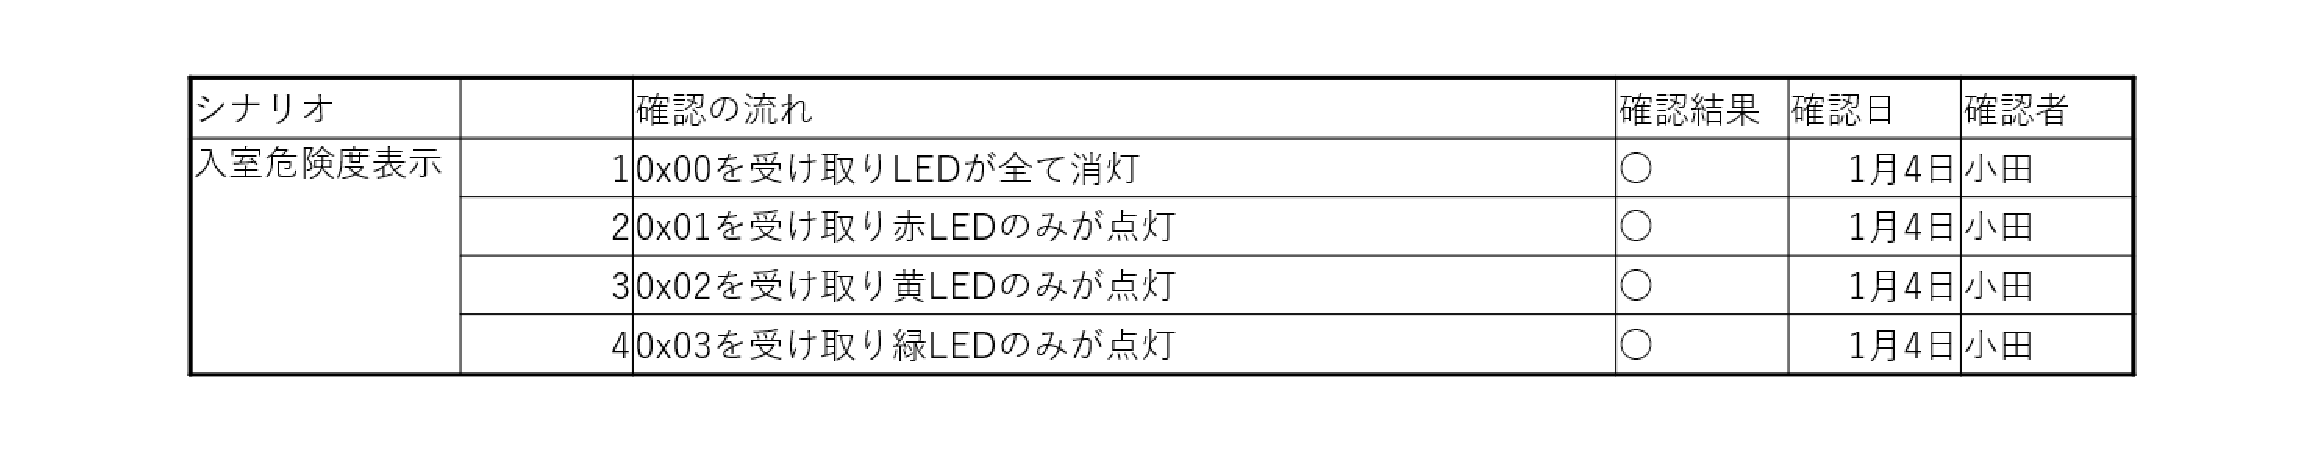
\includegraphics[width=0.9\linewidth]{test/tantaitest_sitsugai_kekka2}
\end{table}

単体テストの実施においては,TWELITEのUART接続を用いてデバイスをPCに接続して行った.
単体テスト項目1~4までPC上から室外デバイスにコマンドを送り,すべて消灯した状態と各入室危険度を表すLEDの制御が正しくできることを確認した.

\subsection{結合テスト}

基本設計の際に挙げた結合テストの項目に従って結合テストを行った.結合テストの結果を表\ref{ketugoutest}に示す.

\begin{table}
	\centering
	\caption{結合テストの結果}
	\label{ketugoutest}
	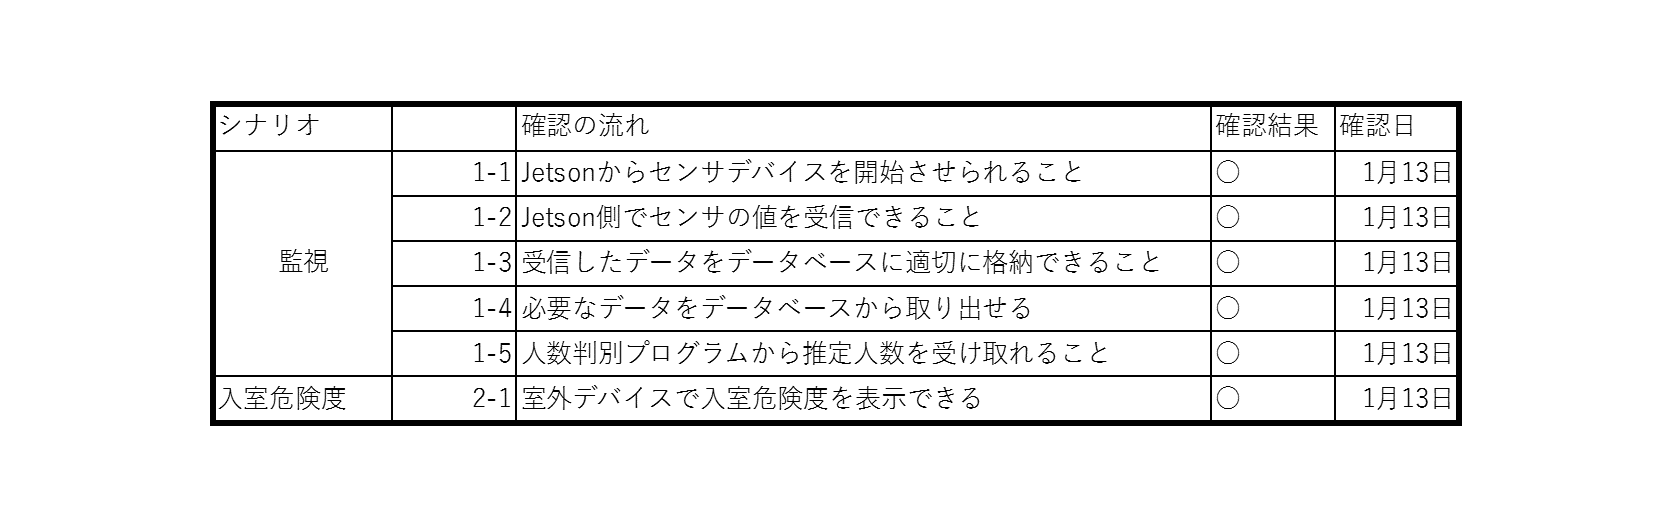
\includegraphics[width=0.9\linewidth]{test/ketugoutest}
\end{table}

結合テストは,環境値評価と人数推定を同一プログラムで行える状態で,データベース操作のプログラムも同一のJetsonで行えるようにして状態で実施した.

項目1-1については,センサデバイスの電源が入っている状態でJetsonの処理プログラムを開始したところ,LEDの状態変化によりセンサデバイスが正しく動作することを確認した.
項目1-2については,Jetsonの処理プログラムを実行することでセンサデバイスから電波を受信していることを確認した.
項目1-3については,処理プログラムの動作中にデータベースに格納された値を定期的に確認し,受信したデータを適切に格納できていることを確認した.
項目1-4については,データベースにデータが格納されている状態から,その値を用いた評価ができていることを確認した.
項目1-5については,プログラムの中で人数推定の結果を正しく受け取れていることを確認した.
項目2-1については,Jetson上で評価した入室危険度に応じて室外デバイスのLEDが正しく点灯していることを確認した.

\subsection{総合テスト}

要求定義の際に挙げた総合テストの項目に従って総合テストを行った.総合テストの結果を表\ref{sougoutest}に示す.

\begin{table}
	\centering
	\caption{総合テストの結果}
	\label{sougoutest}
	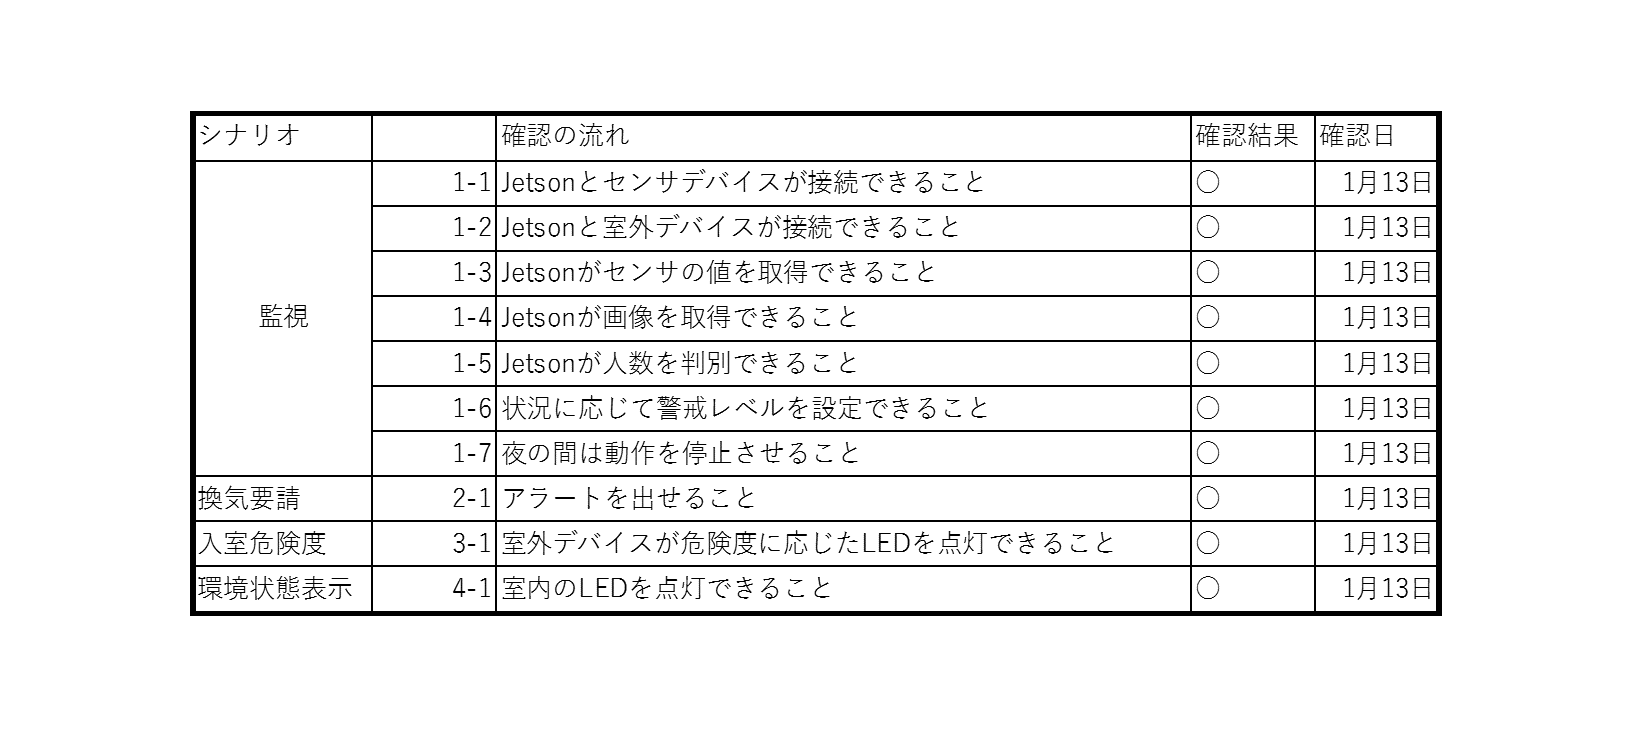
\includegraphics[width=0.9\linewidth]{test/sougoutest}
\end{table}

総合テストは実際にシステムの利用を想定した環境で行った.
項目1-1については,システム実行時にセンサデバイスがJetsonからの開始信号を受け取ることでLEDの状態が変化し,Jetsonとセンサデバイスが接続できていることを確認した.
項目1-2については,システム実行時に室外デバイスのLEDがすべて消灯されるようにすることで,Jetsonと室外デバイスが接続できていることを確認した.
項目1-3については,Jetsonがセンサデバイスから値を受信し,その後の処理に利用できていることを確認した.
項目1-4については,JetsonがWebカメラから画像を取得し,その画像をJetsonと接続したPC上に表示することで正しく画像が取得できていることを確認した.
項目1-5については,人数の異なる集合写真を用いて人数推定を行い,おおむね正しく人数判別できていることを確認した.
項目1-6については,人数の多い集合写真を用いて,室内滞在人数が多く,二酸化炭素濃度値が基準値より高い場合に警戒レベルが上がっていることを確認した.
同様にして,項目2-1と項目4-1について,換気要請のブザーや室内LEDが正しく動作することを確認した.
項目1-7については,設定した時間中,センサ値の取得およびシステムの処理が中断されることを確認した.
項目3-1については,Jetsonが評価した入室危険度に応じて室外デバイスのLEDが正しく点灯することを確認した.